\section{Auswertung}
\label{sec:Auswertung}
\subsection{Messdaten}
\label{sec:Messdaten}
Die bei dem Versuch aufgenommenen Messdaten sind in den Tabellen \ref{tab:mess1} und \ref{tab:mess2} dargestellt. 
\begin{table}[H]
    \centering
        \caption{Die Frequnzverschiebung $\Delta\nu$ bei verschiedenen Pumpleistungen $P$ und Rohrdurchmessern $d_{Rohr}$.}
        \label{tab:mess1}
        \sisetup{table-format=5.0}
        \begin{tabular}{S S S S S S S S S S}
          \toprule
          &
          \multicolumn{9}{c}{$\Delta\nu [\si{\hertz}]$}\\
          \cmidrule(lr){2-10}
          &
          \multicolumn{3}{c}{$d_{Rohr}=\SI{7}{\milli\metre} $}& %\quad\text{Rohr}$} & 
          \multicolumn{3}{c}{$d_{Rohr}=\SI{10}{\milli\metre}$}& %\quad\text{Rohr}$} &
          \multicolumn{3}{c}{$d_{Rohr}=\SI{16}{\milli\metre}$}\\ %\quad\text{Rohr}$} \\
          \cmidrule(lr){2-4}\cmidrule(lr){5-7}\cmidrule(lr){8-10}
          {$P [rpm]$} &
          {$15°$} & {$30°$} & {$45°$} &
          {$15°$} & {$30°$} & {$45°$} &
          {$15°$} & {$30°$} & {$45°$} \\
          \midrule
          6000 & -281 & 439 & -732  & -122 & 208 & -378 & -73 & 85  & -146 \\
          6500 & -317 & 482 & -879  & -134 & 200 & -415 & -73 & 98  & -159 \\
          7000 & -354 & 549 & -1038 & -171 & 281 & -525 & -73 & 110 & -183 \\
          7500 & -385 & 671 & -1172 & -183 & 305 & -635 & -98 & 122 & -220 \\
          8000 & -433 & 708 & -1227 & -195 & 391 & -647 & -98 & 159 & -269 \\
          8500 & -500 & 806 & -1440 & -244 & 415 & -745 & -110& 195 & -330 \\
          \bottomrule
        \end{tabular}
      \end{table}

\begin{table}[H]
  \centering
      \caption{Die Momentangeschwindigkeit $v$ und die Streuintensität $I$ bei Pumpleistungen von $45\%$ und $70\%$.}
      \label{tab:mess2}
      \sisetup{table-format=3.0}
      \begin{tabular}{S S S S S}
        \toprule
        &
        \multicolumn{2}{c}{$P=45\%P_{max}$}&
        \multicolumn{2}{c}{$P=70\%P_{max}$}\\
        \cmidrule(lr){2-3}\cmidrule(lr){4-5}
        {$d_{mess} [\si{\micro\second}]$} &
        {$v [\si{\centi\metre\per\second}]$} & {$I[\si{\square\kilo\volt\per\second}]$} &
        {$v [\si{\centi\metre\per\second}]$} & {$I[\si{\square\kilo\volt\per\second}]$} \\
        \midrule
        12 &     0 & 11  & 0 & 5  \\
        13 &     0 & 33  & 0 & 6  \\
        14 & -28.7 & 73  & 0 & 8  \\
        15 & -35.0 & 108 & 0 & 15 \\
        16 & -36.6 & 125 & 0 & 26 \\
        17 & -31.8 & 111 & 0 & 24 \\
        18 & -31.8 & 117 & 0 & 17 \\
        19 & -31.8 & 470 & 0 & 75 \\
        \bottomrule
      \end{tabular}
    \end{table}

\subsection{Frequnzverschiebung bei verschiedenen Rohrdurchmessern}
\label{sec:a1}
In den Abbildungen \ref{fig:plot1}, \ref{fig:plot2} und \ref{fig:plot3} sind die Messwerte aus Tabelle \ref{tab:mess1} graphisch ausgewertet. 
Dabei sind auf die x-Achsen die Pumpleistungen $P$ und auf die y-Achsen $\Delta\nu/\cos(\alpha)$ aufgetragen, wobei $\alpha$ der jeweilige
Dopplerwinkel aus \ref{sec:vorbereitung} ist. In jeder Abbildung ist dann für jeden Rohrdurchmesser eine lineare Regression eingetragen.
Diese wurde von \textit{nummeric python} \cite{numpy} berechnet und haben die Form 
\begin{equation}
    y=mx+b  . 
    \label{eqn:gerade}
\end{equation}
Die Parameter sind in den Tabellen \ref{tab:params1} - \ref{tab:params3} aufgelistet.

\begin{figure}[H]
  \centering
  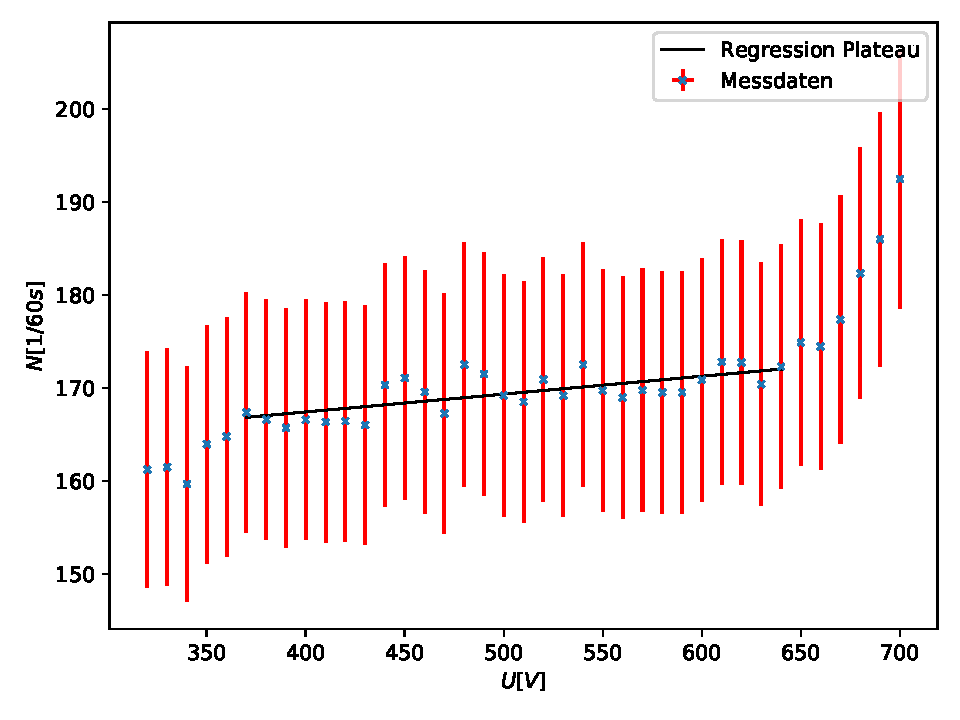
\includegraphics[scale= 0.8]{auswertung/plot1.pdf}
  \caption{$\Delta\nu/\cos(\alpha_{15})$ als Funktion der Pumpleistungen für $\theta=15°$ und für verschiedene Rohrdurchmesser.}
  \label{fig:plot1}
\end{figure}
\begin{table}[H]
  \centering
      \caption{Die Parameter der linearen Regressionen in Abbildung \ref{fig:plot1}.}
      \label{tab:params1}
      \sisetup{table-format=2.3}
      \begin{tabular}{S S @{${}\pm{}$} S S @{${}\pm{}$} S}
        \toprule
        {$d_{Rohr} [\si{\milli\metre}]$} & \multicolumn{2}{c}{$a [\si{\hertz}/\text{rpm}]$} & \multicolumn{2}{c}{$b [\si{\kilo\hertz}]$} \\
        \midrule
        7  & -0.488 & 0.035 &  1.35 & 0.25 \\
        10 & -0.267 & 0.030 &  0.92 & 0.22 \\
        16 & -0.094 & 0.019 &  0.18 & 0.14 \\
        \bottomrule
     \end{tabular}
  \end{table}
\begin{figure}[H]
  \centering
  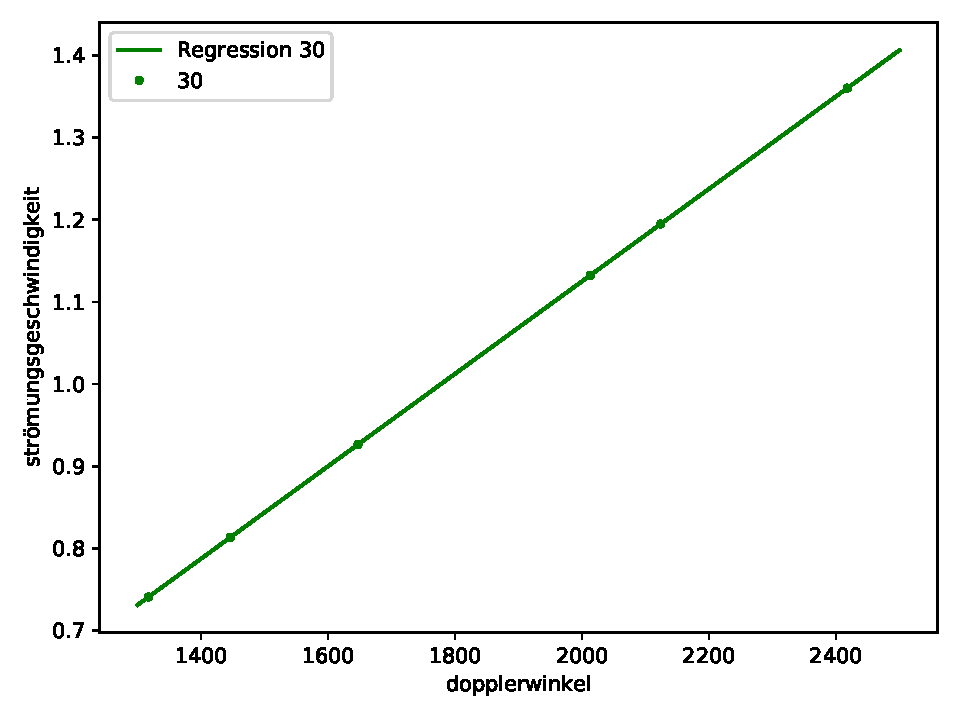
\includegraphics[scale= 0.8]{auswertung/plot2.pdf}
  \caption{$\Delta\nu/\cos(\alpha_{30})$ als Funktion der Pumpleistungen für $\theta=30°$ und für verschiedene Rohrdurchmesser.}
  \label{fig:plot2}
\end{figure}
\begin{table}[H]
  \centering
      \caption{Die Parameter der linearen Regressionen in Abbildung \ref{fig:plot2}.}
      \label{tab:params2}
      \sisetup{table-format=2.3}
      \begin{tabular}{S S @{${}\pm{}$} S S @{${}\pm{}$} S}
        \toprule
        {$d_{Rohr} [\si{\milli\metre}]$} & \multicolumn{2}{c}{$a [\si{\hertz}/\text{rpm}]$} & \multicolumn{2}{c}{$b [\si{\kilo\hertz}]$} \\
        \midrule
        7  & 0.452 & 0.031  & -1.45 & 0.23 \\
        10 & 0.280 & 0.034  & -1.13 & 0.25 \\
        16 & 0.128 & 0.018  & -0.54 & 0.13 \\
        \bottomrule
     \end{tabular}
  \end{table}
\begin{figure}[H]
  \centering
  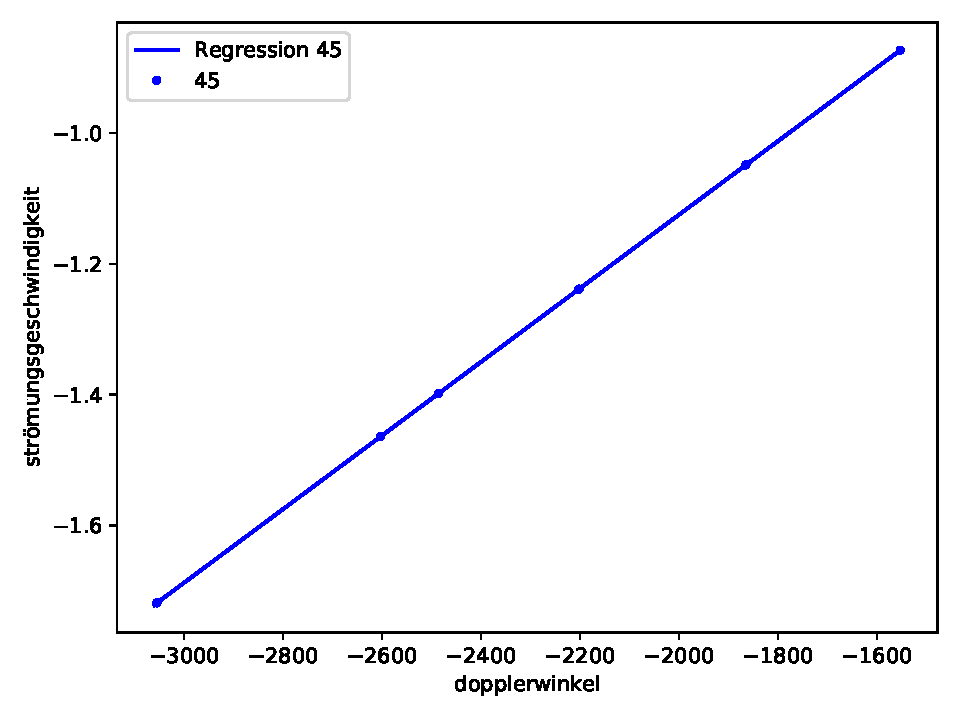
\includegraphics[scale= 0.8]{auswertung/plot3.pdf}
  \caption{$\Delta\nu/\cos(\alpha_{45})$ als Funktion der Pumpleistungen für $\theta=45°$ und für verschiedene Rohrdurchmesser.}
  \label{fig:plot3}
\end{figure}
\begin{table}[H]
\centering
    \caption{Die Parameter der linearen Regressionen in Abbildung \ref{fig:plot3}.}
    \label{tab:params3}
    \sisetup{table-format=2.3}
    \begin{tabular}{S S @{${}\pm{}$} S S @{${}\pm{}$} S}
      \toprule
      {$d_{Rohr} [\si{\milli\metre}]$} & \multicolumn{2}{c}{$a [\si{\hertz}/\text{rpm}]$} & \multicolumn{2}{c}{$b [\si{\kilo\hertz}]$} \\
      \midrule
      7  & -0.57  & 0.04   &  1.85 & 0.26 \\
      10 & -0.320 & 0.028  &  1.14 & 0.21 \\
      16 & -0.156 & 0.019  &  0.67 & 0.14 \\
      \bottomrule
   \end{tabular}
\end{table}

\subsection{Strömungsprofil}
\label{sec:a2}
Die Messwerte aus Tabelle \ref{tab:mess2} sind in den Abbildungen \ref{fig:plot4} und \ref{fig:plot5} dargestellt. Dabei entsprechen die 
Pumpleistungen in Prozent
\begin{align*}
  P_{45}&=45\%P_{max}=3870\text{rpm}\\
  P_{70}&=70\%P_{max}=6000\text{rpm}.
\end{align*}
In Abbildung \ref{fig:plot4} ist die Messtiefe $\mu$ gegen die Momentangeschwindigkeit $v_ström$ aufgetragen. Die Regression ist dabei wieder
der Form von Gleichung \eqref{eqn:gerade}. Die Parameter sind in Tabelle \ref{tab:params4} aufgelistet. Aufgrund technischer Schwierigkeiten
(vgl.Kapitel \ref{sec:Diskussion}) ist sind für die Daten von $P_{70}$ zwei Regressionen erstellt worden. Die graue Regression ist dabei aus allen 
Messdaten berechnet, bei der roten Gerade sind jene Werte aus der Berechnung ausgeschlossen, für welche $v_{stroem}=\SI{0}{\metre\per\second}$
ist. Diese Werte sind zudem noch mit einem Stern markiert. 
\begin{figure}[H]
  \centering
  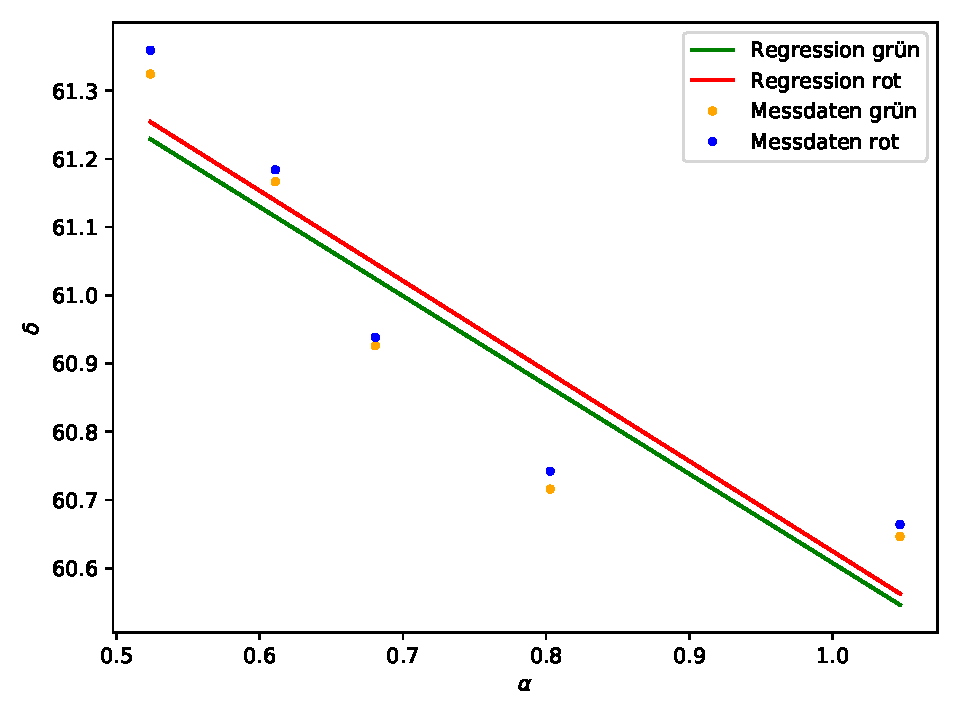
\includegraphics[scale= 0.8]{auswertung/plot4.pdf}
  \caption{Die Momentangeschwindigkeit $v_{stroem}$ als Funktion der Messtiefe $\mu$ für verschiedene Pumpleistungen.}
  \label{fig:plot4}
\end{figure}
\begin{table}[H]
\centering
    \caption{Die Parameter der linearen Regressionen in Abbildung \ref{fig:plot4}. Die letzt Zeile enthält die bereinigte Regression.}
    \label{tab:params4}
    \sisetup{table-format=1.3}
    \begin{tabular}{S[table-format=4.0] S @{${}\pm{}$} S S @{${}\pm{}$} S}
      \toprule
      {$P [\text{rpm}]$} & \multicolumn{2}{c}{$a [\si{\kilo\metre\per\square\second}]$} & \multicolumn{2}{c}{$b [\si{\metre\per\second}]$} \\
      \midrule
      3870 &  0.00 & 0.00 & 0.000  & 0.000 \\
      6000 & -4.73 & 1.69 & 0.048  & 0.026 \\
      6000 & -0.03 & 0.75 & -0.032 & 0.012 \\
      \bottomrule
   \end{tabular}
\end{table}
\noindent
Die Streuintensität $I$ ist in Abbildung \ref{fig:plot5} gegen die Messtiefe $\mu$ aufgetragen. Auch die Regression der Messdaten von $P_{70}$
wurde zweimal durchgeführt, in grau mit allen Daten und in rot mit allen Daten, außer dem mit Stern markierten Messwert (vgl. Kapitel\ref{sec:Diskussion}).
Die Regressionen sind wieder linear und die Parameter sind in Tabelle \ref{tab:params5} aufgeführt.

\begin{figure}[H]
  \centering
  \includegraphics[scale= 0.8]{auswertung/plot5.pdf}
  \caption{Die Streuintensität $I$ als Funktion der Messtiefe $\mu$ für verschiedene Pumpleistungen.}
  \label{fig:plot5}
\end{figure}
\begin{table}[H]
\centering
    \caption{Die Parameter der linearen Regressionen in Abbildung \ref{fig:plot4}. Die letzt Zeile enthält die bereinigte Regression.}
    \label{tab:params5}
    \sisetup{table-format=3.1}
    \begin{tabular}{S[table-format=4.0] S[table-format=2.2] @{${}\pm{}$} S[table-format=2.2] S[table-format=4.1] @{${}\pm{}$} S}
      \toprule
      {$P [\text{rpm}]$} & \multicolumn{2}{c}{$a [\si{\giga\square\volt\per\square\second}]$} & \multicolumn{2}{c}{$b [\si{\square\kilo\volt\per\square\second}]$} \\
      \midrule
      3870 &  7.19 &  2.42 & -89.5 &  37.9 \\
      6000 & 44.81 & 15.32 & -563.5 & 240.0 \\
      6000 & 18.79 & 3.99  &  187.9 &  39.9 \\
      \bottomrule
   \end{tabular}
\end{table}
